\documentclass{article}
\usepackage{amsmath, amssymb}
\usepackage{graphicx}
\usepackage{tikz}
\usepackage{pgfplots}
\pgfplotsset{compat=1.17}
\usepackage{hyperref}
\usepackage{caption}
\usepackage{subcaption}

\begin{document}

\title{Analyzing the Curvature of a Hyperbolic Paraboloid Using Partial Derivatives}
\author{Roxy Rahimi}
\date{October 5, 2024}

\maketitle

\section*{Introduction}

The hyperbolic paraboloid is a saddle-shaped surface, famously resembling a Pringle chip, commonly studied in multivariable calculus and differential geometry. It is defined by the equation:

\[
z = \frac{x^2}{a^2} - \frac{y^2}{b^2}
\]

Understanding the curvature of this surface involves analyzing its second partial derivatives. This document explores how the signs of these derivatives affect concavity in different directions and delves into the significance of the mixed partial derivatives.

\section{Second Partial Derivatives and Concavity}

The second partial derivatives \( f_{xx} \) and \( f_{yy} \) of a function \( f(x, y) \) provide insight into its concavity along the \( x \) and \( y \) axes, respectively.

\subsection{Case 1: \( f_{xx} > 0 \) and \( f_{yy} < 0 \)}

When \( f_{xx} > 0 \), the function is concave up in the \( x \)-direction. Conversely, \( f_{yy} < 0 \) indicates concave down in the \( y \)-direction. For a hyperbolic paraboloid, this results in a surface that curves upward along \( x \) and downward along \( y \).

\subsubsection*{Work}

Consider \( f(x, y) = x^2 - y^2 \):

\[
f_{xx} = \frac{\partial^2 f}{\partial x^2} = 2 > 0, \quad f_{yy} = \frac{\partial^2 f}{\partial y^2} = -2 < 0
\]

\subsubsection*{Visualization}

\begin{figure}[h]
\centering
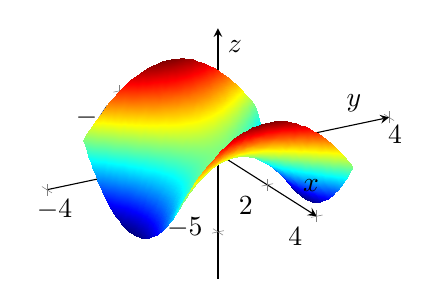
\begin{tikzpicture}
  \begin{axis}[
    axis lines=middle, % Place axes in the middle
    xlabel={$x$}, ylabel={$y$}, zlabel={$z$}, % Axis labels
    domain=-2:2,
    y domain=-2:2,
    samples=40,
    samples y=40,
    z buffer=sort,
    colormap/jet,
    point meta min=-4, point meta max=4,
    view={60}{30},
    xmin=-4, xmax=4, % Extend x-axis limits
    ymin=-4, ymax=4, % Extend y-axis limits
    zmin=-8, zmax=8, % Extend z-axis limits
  ]
    \addplot3[surf, shader=interp]
    {x^2 - y^2};
  \end{axis}
\end{tikzpicture}
\caption{Custom hyperbolic paraboloid (Pringle shape) showing concave up in \( x \)-direction as its partial derivative is positive and concave down in \( y \)-direction as its partial derivative is negative}
\label{fig:custom_pringle_long_axes}
\end{figure}

\subsection{Case 2: \( f_{xx} < 0 \) and \( f_{yy} > 0 \)}

Here, \( f_{xx} < 0 \) means the function is concave down in \( x \)-direction, and \( f_{yy} > 0 \) implies concave up in \( y \)-direction.

\subsubsection*{Work}

Consider \( f(x, y) = -x^2 + y^2 \):

\[
f_{xx} = -2 < 0, \quad f_{yy} = 2 > 0
\]

\subsubsection*{Visualization}



\begin{figure}[h]
\centering
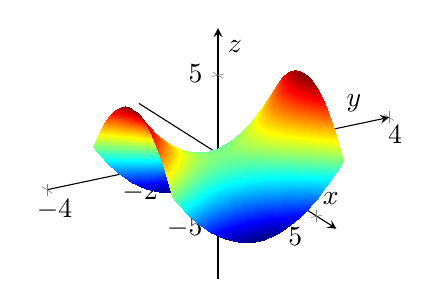
\begin{tikzpicture}
  \begin{axis}[
    axis lines=middle,
    xlabel={$x$}, ylabel={$y$}, zlabel={$z$},
    domain=-2:2,
    y domain=-2:2,
    samples=40,
    samples y=40,
    z buffer=sort,
    colormap/jet,
    point meta min=-4, point meta max=4,
    view={60}{30},
    xmin=-4, xmax=6,
    ymin=-4, ymax=4,
    zmin=-8, zmax=8,
  ]
    \addplot3[surf, shader=interp]
    {-x^2 + y^2};
  \end{axis}
\end{tikzpicture}
\caption{Custom hyperbolic paraboloid showing concave down in \( x \)-direction as its partial derivative is negative and concave up in \( y \)-direction as its partial derivative is positive}
\label{fig:custom_pringle_inverse_long_axes}
\end{figure}

\section{Equality and Interpretation of Mixed Partial Derivatives}

In continuous functions, the mixed partial derivatives are equal:

\[
f_{xy} = f_{yx}
\]

These derivatives represent the rate of change of the slope in one direction as you move along the other.
\section{consider the hyperbolic paraboloid given by:}

\[
z = c^2 \left( \frac{x^2}{a^2} - \frac{y^2}{b^2} \right).
\]

We want to find the mixed partial derivatives \( f_{xy} \) and \( f_{yx} \) and show that they are equal to zero.

\subsection{Step 1: Find the First Partial Derivatives}

find the partial derivative of \( z \) with respect to \( x \):

\[
f_x = \frac{\partial z}{\partial x} = c^2 \cdot \frac{\partial}{\partial x} \left( \frac{x^2}{a^2} - \frac{y^2}{b^2} \right).
\]

\[
f_x = c^2 \cdot \frac{2x}{a^2} = \frac{2c^2 x}{a^2}.
\]

\subsection{Step 2: Find the Mixed Partial Derivative \( f_{xy} \)}

find the partial derivative of \( f_x \) with respect to \( y \):

\[
f_{xy} = \frac{\partial}{\partial y} \left( \frac{2c^2 x}{a^2} \right).
\]

\[
f_{xy} = 0.
\]

\subsection{Step 3: Find the First Partial Derivative with Respect to \( y \)}

find the partial derivative of \( z \) with respect to \( y \):

\[
f_y = \frac{\partial z}{\partial y} = c^2 \cdot \frac{\partial}{\partial y} \left( \frac{x^2}{a^2} - \frac{y^2}{b^2} \right).
\]

\[
f_y = -c^2 \cdot \frac{2y}{b^2} = -\frac{2c^2 y}{b^2}.
\]

\subsection*{Step 4: Find the Mixed Partial Derivative \( f_{yx} \)}

find the partial derivative of \( f_y \) with respect to \( x \):

\[
f_{yx} = \frac{\partial}{\partial x} \left( -\frac{2c^2 y}{b^2} \right).
\]

\[
f_{yx} = 0.
\]

\section*{Conclusion}

It is proven that

\[
f_{xy} = 0 \quad \text{and} \quad f_{yx} = 0.
\]

Therefore, for the hyperbolic paraboloid given by \( \frac{z}{c^2} = \frac{x^2}{a^2} - \frac{y^2}{b^2} \), the mixed partial derivatives \( f_{xy} \) and \( f_{yx} \) are both zero. **this will always be the case  


\section{Mixed Partial Derivative \( f_{xy} \) in Hyperbolic Paraboloids}

\subsection{Significance of Different Signs of \( f_{xy} \)}

A positive \( f_{xy} \) or \( f_{yx} \)means that the curvature of one direction depends on the position in the other direction since these derivatives represent the rate of change of the slope in one direction as you move along the other. When \( f_{xy} \) is positive, \( x \) and \( y \) increase or decrease together results in an increasing slope. When \( f_{xy} \) is negative, it means that the slope in \( x \) changes as \( y \) changes, and vice versa
When \( f_{xy} \) is positive or negative, it shows a twisting surface. 

Imagine a flat sheet of paper that is twisted by holding opposite corners and rotating them in opposite directions. 

Doesn't this show how the rate of change of the slope in one direction changes as you move the other? On the other hand, image pressing down on the center of a paper without moving the edges. This causes the sheet of paper to bend uniformly, and to not twist. 

** I believe this means that with that when there is twisting (meaning the mixed partial is either negative or positive) the contour lines may curve or skew. However, when there is no twisting (meaning the mixed partial is equal to 0) the contour lines are symmetrical. 
You can also analyze slices of a surface at constant x or y to observe how the curvature changes. This is what \( f_{xy} = 0 \) and \( f_{yx} = 0 \) measure.



\subsection{\( f_{xy} = 0 \)}

So, when \( f_{xy} = 0 \), the surface doesn't twist in the mixed direction. This is because the curvature along x and y are independent. The curvature in the y direction is independent of x. The surface curves upwards or downwards along each axis without being influenced by the other axis - which makes sense when we think about the typical pringle shape. In other words, the slope in the x direction remains constant as y varies. There is no twisting or warping of the surface caused by the interaction of x and y. 

This explanation perfectly aligns with the hyperbolic paraboloid shape. The cross sections of the shape do not warp or deviate. The contour lines should be symmetrical so therefore the curvature in the y direction is independent of x and vice versa. 

\subsection{Consider a function such as \( z = xy \)}
\( f_{xy} = 1 \)
\newline
\( f_{yx} = 1 \)
\newline
this means that the rate at which the slope of the x direction changes as you move along the y direction warps because the slope in one direction changes as you move along the other direction. 

In other words, as y increases, the slope of the line in the x direction increases. As x increases, the slope of the line in the y direction increases. 



\end{document}
